\documentclass[12pt, a4paper]{report}
\usepackage[top=1cm, left=1cm, right=1cm]{geometry}

\usepackage[utf8]{inputenc}
\usepackage[russian]{babel}

\usepackage{array}
\newcolumntype{M}[1]{>{\centering\arraybackslash}m{#1}}

\usepackage{hyperref}
\hypersetup{
	colorlinks,
	citecolor=black,
	filecolor=black,
	linkcolor=black,
	urlcolor=black
}

\usepackage{sectsty}
\allsectionsfont{\centering}

\usepackage{indentfirst}
\setlength\parindent{24pt}

\usepackage{algorithm}
\usepackage[noend]{algpseudocode}

\usepackage{listings}
\usepackage{xcolor}
\definecolor{codegreen}{rgb}{0,0.6,0}
\definecolor{codegray}{rgb}{0.5,0.5,0.5}
\definecolor{codepurple}{rgb}{0.58,0,0.82}
\definecolor{backcolour}{rgb}{0.95,0.95,0.92}
\lstdefinestyle{mystyle}{
    backgroundcolor=\color{backcolour},
    commentstyle=\color{codegreen},
    keywordstyle=\color{magenta},
    numberstyle=\normalsize\color{codegray},
    stringstyle=\color{codepurple},
    basicstyle=\ttfamily\footnotesize,
    breakatwhitespace=false,
    breaklines=true,
    captionpos=b,
    keepspaces=true,
    numbers=left,
    numbersep=5pt,
    showspaces=false,
    showstringspaces=false,
    showtabs=false,
    tabsize=2
}

\usepackage{graphicx}
\graphicspath{ {plots/pictures/}{assets/pictures} }

\begin{document}
	\begin{titlepage}
		\begin{center}
			\large \textbf{Министерство науки и высшего образования Российской Федерации} \\
			\large \textbf{Федеральное государственное бюджетное образовательное учреждение высшего образования} \\
			\large \textbf{«Российский химико-технологический университет имени Д.И. Менделеева»} \\

			\vspace*{4cm}
			\LARGE \textbf{ОТЧЕТ ПО ЛАБОРАТОРНОЙ РАБОТЕ №7}

			\vspace*{4cm}
			\begin{flushright}
				\Large
				\begin{tabular}{>{\raggedleft\arraybackslash}p{9cm} p{10cm}}
					Выполнил студент группы КС-36: & Золотухин А.А. \\
					Ссылка на репозиторий: & https://github.com/ \\
					& MUCTR-IKT-CPP/ \\
					& ZolotukhinAA\_36\_ALG \\
					Принял: & Крашенников Роман Сергеевич \\
					Дата сдачи: & 14.04.2025 \\
				\end{tabular}
			\end{flushright}

			\vspace*{6cm}
			\Large \textbf{Москва \\ 2025}
		\end{center}
	\end{titlepage}

	\tableofcontents
	\thispagestyle{empty}
	\newpage

	\pagenumbering{arabic}

	\section*{Описание задачи}
	\addcontentsline{toc}{section}{Описание задачи}
	\large
	В рамках лабораторной рабоыт необходимо изучить дерево поиска: \textit{Декартово дерево}. \par
	Для этого его потребуется реализовать и сравнить в работе с реализованным \textit{AVL-деревом}. Для анализа работы алгоритма понадобиться провести серии тестов:
	\begin{itemize}
		\item в одной серии тестов проводится \underline{50} повторений;
		\item требуется провести серии тестов для \textit{N} = \underline{$2^i$}, при этом \textit{i} от \underline{10} до \underline{18} включительно.
	\end{itemize}
	\par
	В рамках одной серии понадобится сделать следующее:
	\begin{itemize}
		\item сгенерировать \textit{N} случайных значений;
		\item заполнить два дерева \textit{N} количеством элементов в одинаковом порядке;
		\item для каждой из серий тестов замерить максимальную глубину полученного дерева;
		\item для каждого дерева после заполнения провести \underline{1000} операций вставки и замерить время;
		\item для каждого дерева после заполнения провести \underline{1000} операций удаления и замерить время;
		\item для каждого дерева после заполнения провести \underline{1000} операций поиска и замерить время;
		\item для каждого дерева замерить глубины всех веток дерева.
	\end{itemize}
	\par
	Для анализа структуры потребуется построить следующие график:
	\begin{itemize}
		\item график зависимости среднего времени вставки от количества элементов в изначальном дереве для декартова и AVL деревьев;
		\item график зависимости среднего времени удаления от количества элементов в изначальном дереве для декартова и AVL деревьев;
		\item график зависимости среднего времени поиска от количества элементов в изначальном дереве для декартова и AVL деревьев;
		\item график максимальной высоты полученного дерева в зависимости от \textit{N};
		\item гистограмму среднего распределения максимальной высоты для последней серии тестов для AVL и декартова дерева;
		\item гистограмму среднего распределения высот веток для последней серии тестов для AVL и декартова дерева.
	\end{itemize}
	\par
	\textbf{Дополнительное задание}:
	\begin{itemize}
		\item аналогичная серия тестов и сравнение её для отсортированного заранее набора данных;
		\item реализовать \textit{красно-чёрное дерево} и провести все те же проверки с ним.
	\end{itemize}
	
	\newpage

	\section*{Описание метода/модели}
	\addcontentsline{toc}{section}{Описание метода/модели}
	\large
	\textbf{Декартово дерево} - двоичное дерево поиска, которое является достаточно популярной и простой реализацией самобалансирующегося варианта дерева. Декартово дерево в каждом узле помимо ключа, хранит так же приоритет узла, который отражает позицию элемента в такой структуре данных, как куча. \textbf{Куча} - древовидная структура, у которой родитель дерева боле всех его потомков (или меньше). По этой причине декартово дерево часто называют \textit{treap} = \textit{tree} + \textit{heap}. Такое дерево называется декартовым по той причине, что его узлы можно уложить на координатной плоскости, где \textit{x} - ключ, а \textit{y} - приоритет. \par
	\textbf{Построение декартового дерева}. Потребуется:
	\begin{enumerate}
		\item \textit{множество ключей} - те значения, которые есть в наших данных, по которым мы и хотим построить декартово дерево поиска;
		\item \textit{множество приоритетов} - случайная величина, которую мы можем как генерировать самостоятельно, так и брать из поступающих нам данных, связанных с ключами.
	\end{enumerate}
	\par
	\textit{Два особенных момента}:
	\begin{itemize}
		\item одинаковые ключи следует хранить либо только в правом поддереве, либо только в левом, и тогда они не будут доставлять проблем;
		\item одинаковых приоритетов стоит избегать, в идеале генерировать случайные числа от \textit{0} до \textit{1}, но, если нужно, можно и случайное целочисленное число.
	\end{itemize}
	\textbf{Две важные операции} для работы с декартовым деревом:

	\newpage

	\section*{Выполнение задачи}
	\addcontentsline{toc}{section}{Выполнение задачи}
	AVL, декартово и красно-чёрное деревья реализованы на языке \textit{C++}. Построение графиков проводились с помощью программы \textit{GNUplot}.

	\newpage
	\vfill

	\begin{figure}[h]
		\centering
		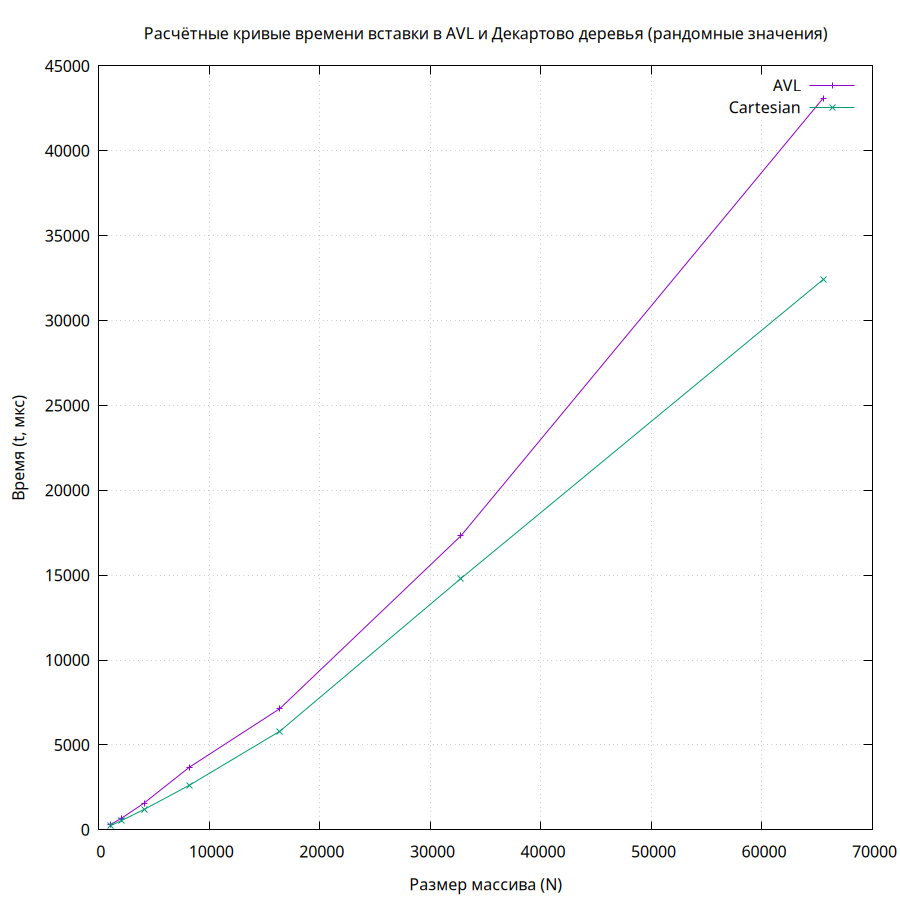
\includegraphics[width=250pt]{insert_random.png}
		\caption{Расчётные кривые времени вставки в AVL, Декартово и Красно-чёрное деревья (рандомные значения).}
	\end{figure}
	\begin{figure}[h]
		\centering
		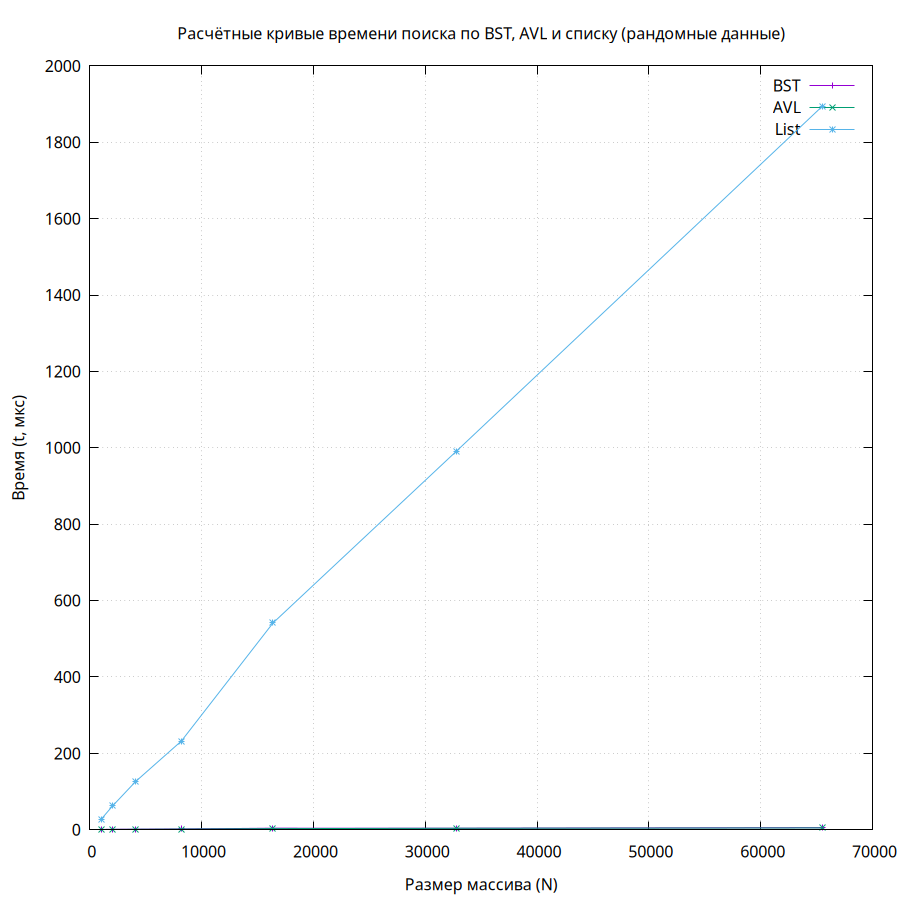
\includegraphics[width=250pt]{search_random.png}
		\caption{Расчётные кривые времени поиска по AVL, Декартово и Красно-чёрное деревьям (рандомные данные).}
	\end{figure}
	\begin{figure}[h]
		\centering
		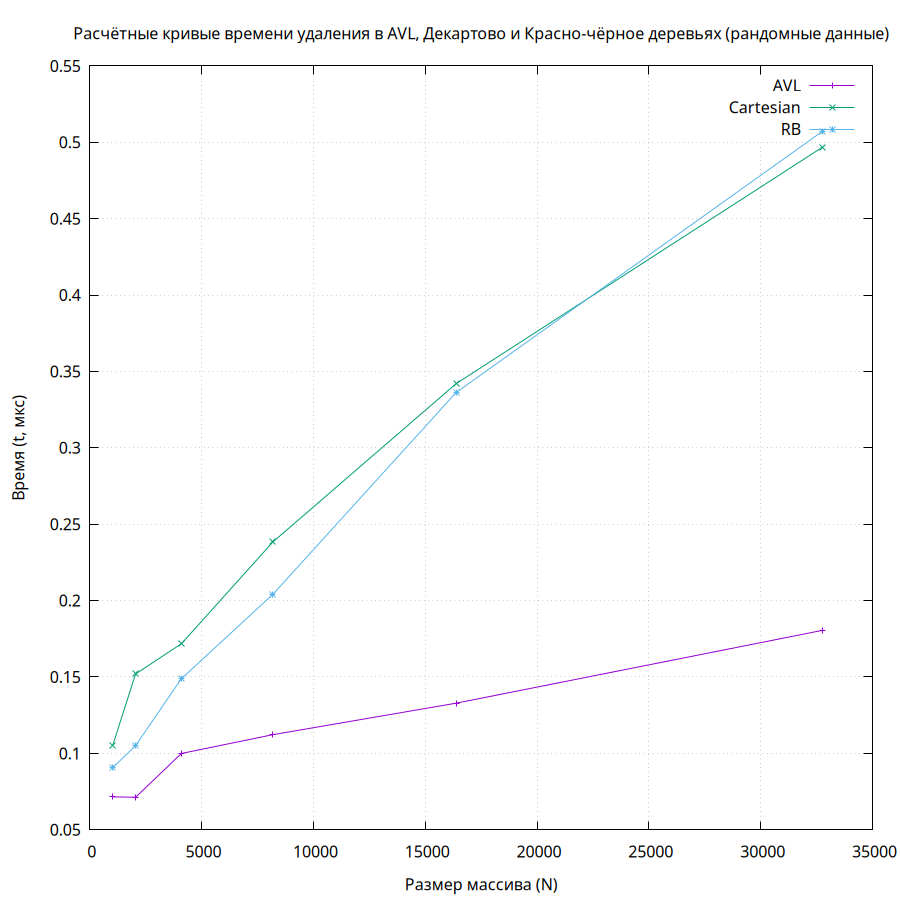
\includegraphics[width=250pt]{delete_random.png}
		\caption{Расчётные кривые времени удаления в AVL, Декартово и Красно-чёрное деревьях (рандомные данные).}
	\end{figure}
	\begin{figure}[h]
		\centering
		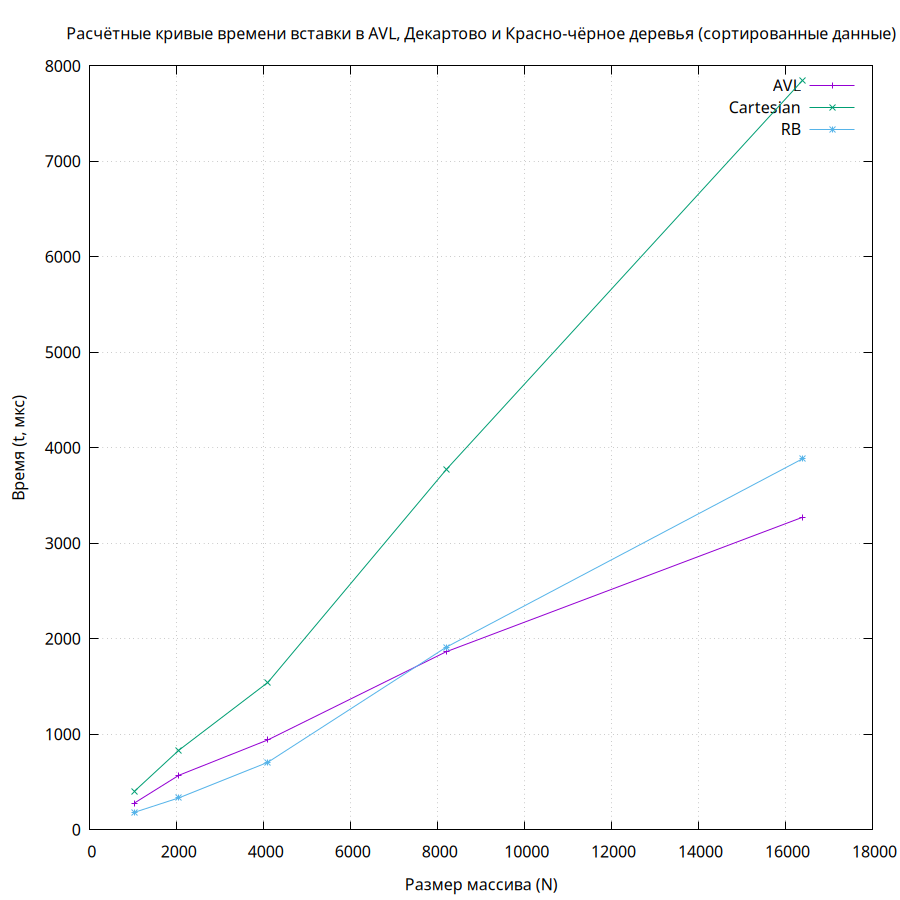
\includegraphics[width=250pt]{insert_sorted.png}
		\caption{Расчётные кривые времени вставки в AVL, Декартово и Красно-чёрное деревья (сортированные данные).}
	\end{figure}
	\begin{figure}[h]
		\centering
		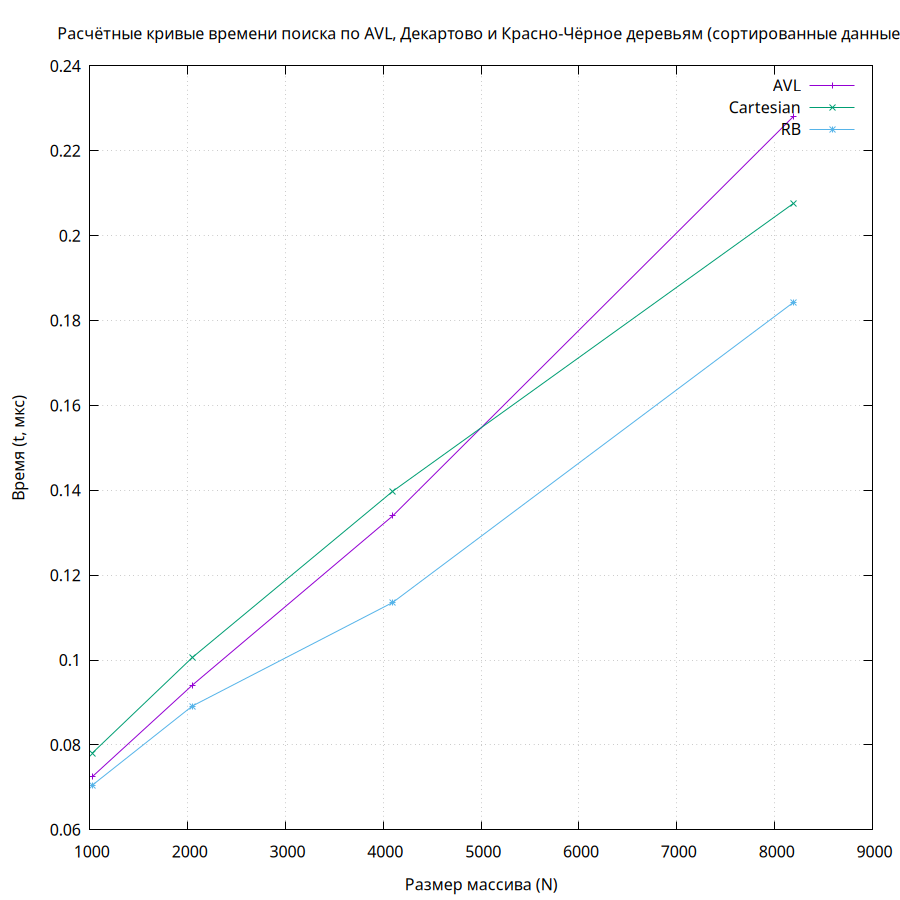
\includegraphics[width=250pt]{search_sorted.png}
		\caption{Расчётные кривые времени поиска по AVL, Декартово и Красно-Чёрное деревьям (сортированные данные).}
	\end{figure}
	\begin{figure}[h]
		\centering
		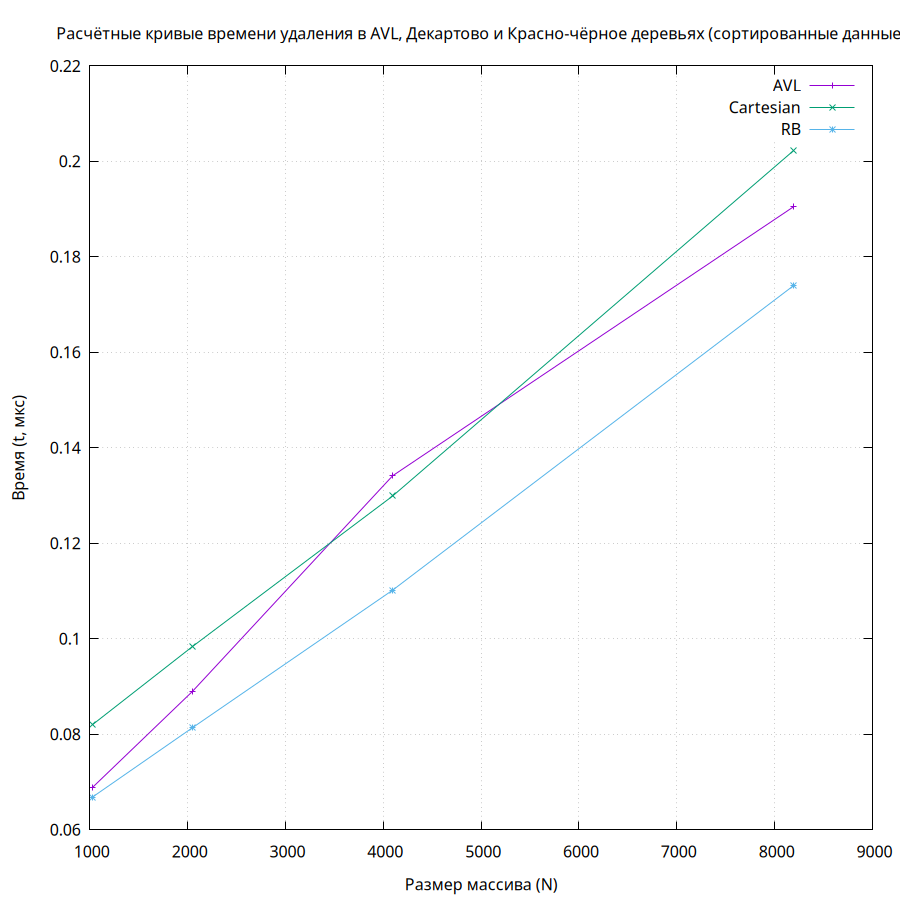
\includegraphics[width=250pt]{delete_sorted.png}
		\caption{Расчётные кривые времени удаления в AVL, Декартово и Красно-чёрное деревьях (сортированные данные).}
	\end{figure}	
	\begin{figure}[h]
		\centering
		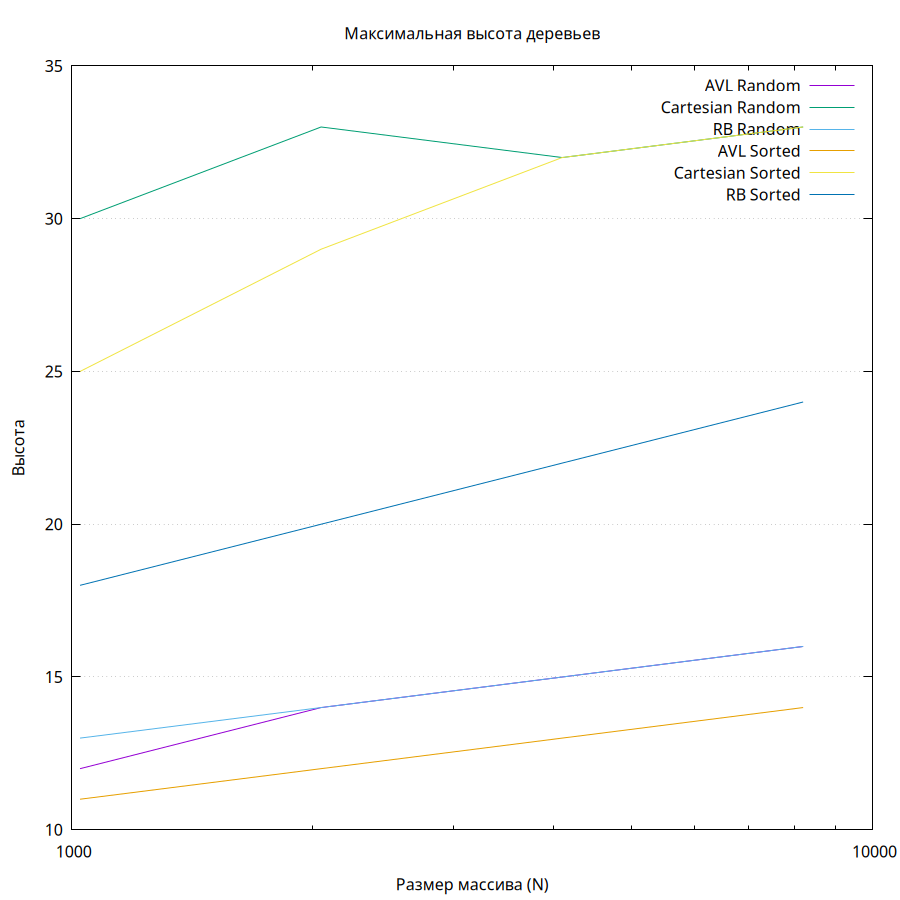
\includegraphics[width=250pt]{max_height.png}
		\caption{Расчётные кривые максимальной высоты в AVL, Декартово и Красно-чёрное деревьях.}
	\end{figure}
	\begin{figure}[h]
		\centering
		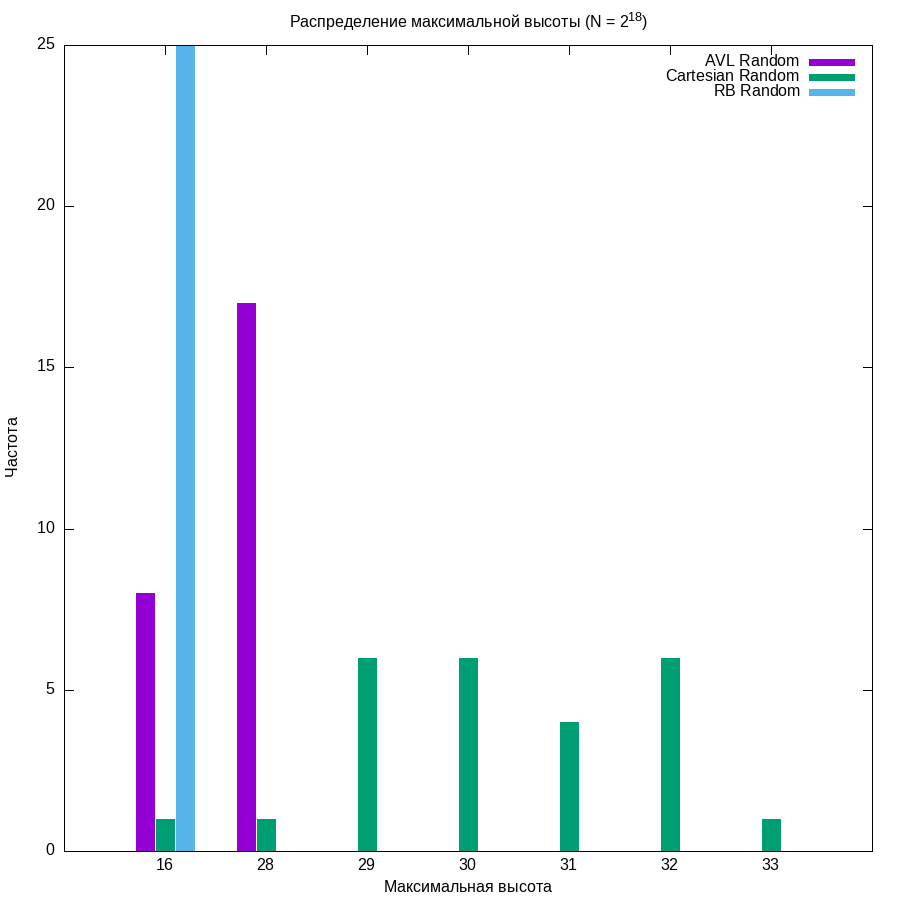
\includegraphics[width=250pt]{max_height_distribution.png}
		\caption{Распределение максимальной высоты ($N = 2^{18}$) (рандомные данные).}
	\end{figure}	
	\begin{figure}[h]
		\centering
		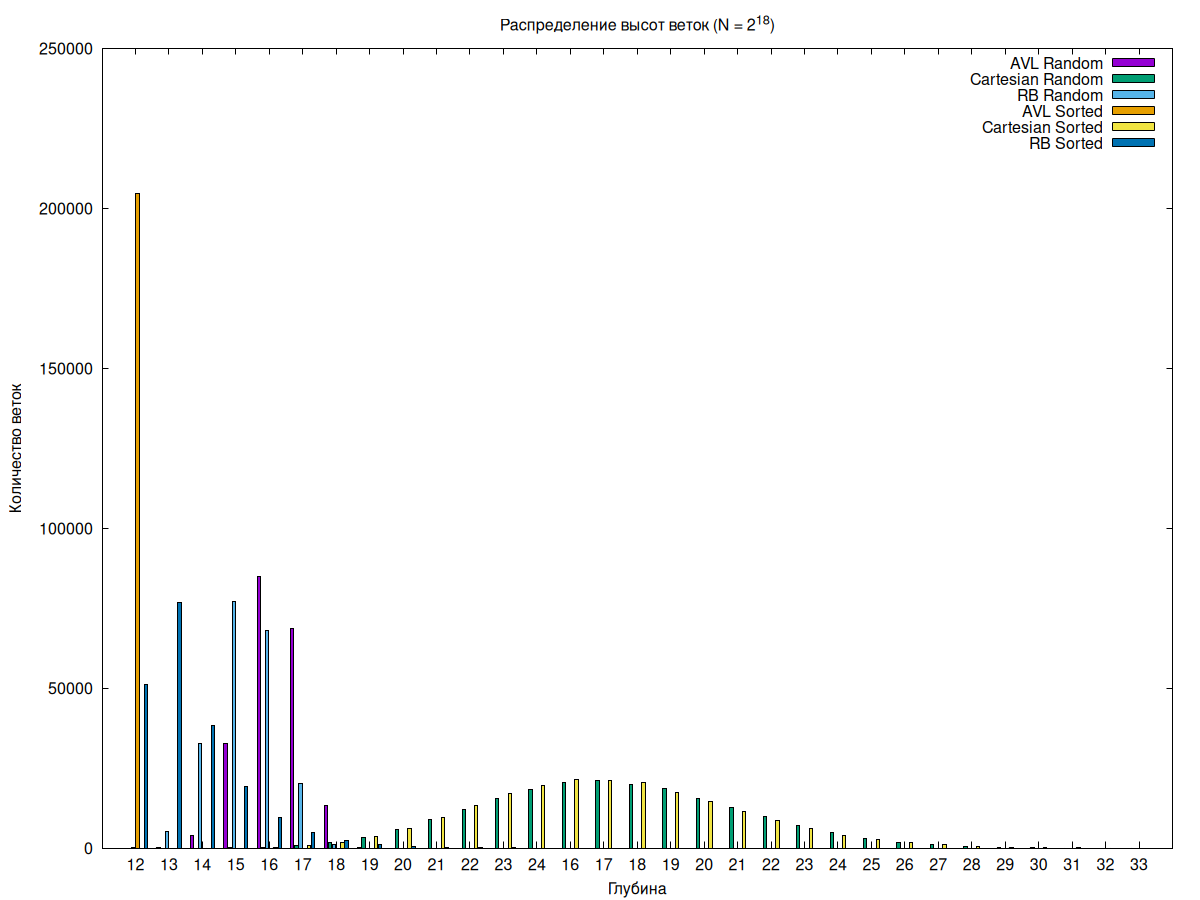
\includegraphics[width=250pt]{depths_distribution.png}
		\caption{Распределение высот веток ($N = 2^{18}$) (рандомные данные).}
	\end{figure}
\end{document}
